%\documentclass{llncs}
\documentclass[journal, letterpaper]{IEEEtran}
%\documentclass{scrartcl}


\usepackage[ngerman,english]{babel}
%\usepackage[latin1]{inputenc}
\usepackage[utf8]{inputenc}
\usepackage[T1]{fontenc}
\usepackage{amsmath}
\usepackage{amsthm}
\usepackage{amsfonts}
\usepackage{tikz}
\usepackage{verbatim}
\usepackage{subcaption}
\usepackage{algorithm}
\usepackage{algorithmic}
\usepackage[pdftex]{hyperref}

\renewcommand{\algorithmicrequire}{\textbf{Input:}}
\renewcommand{\algorithmiccomment}[1]{\ \ // #1} % C-like // Comments

\hyphenation{render}

% No clubs and widows allowed
\clubpenalty10000
\widowpenalty10000
\displaywidowpenalty=10000

\begin{document}

%\title{Simulating elastic spheres without external forces}
%\subtitle{Project 1 for class CS6491 Computer Graphics}
\title{Procedural Terrain \\
	{\large Final project for class CS6491 Computer Graphics}}
%\author{Sebastian Weiss}
\author{Sebastian Weiss \\ \today}
%\date{\today}

\maketitle

%\begin{tikzpicture}[remember picture,overlay]
%   \node[anchor=north east,inner sep=0pt] at (current page.north east)
%              {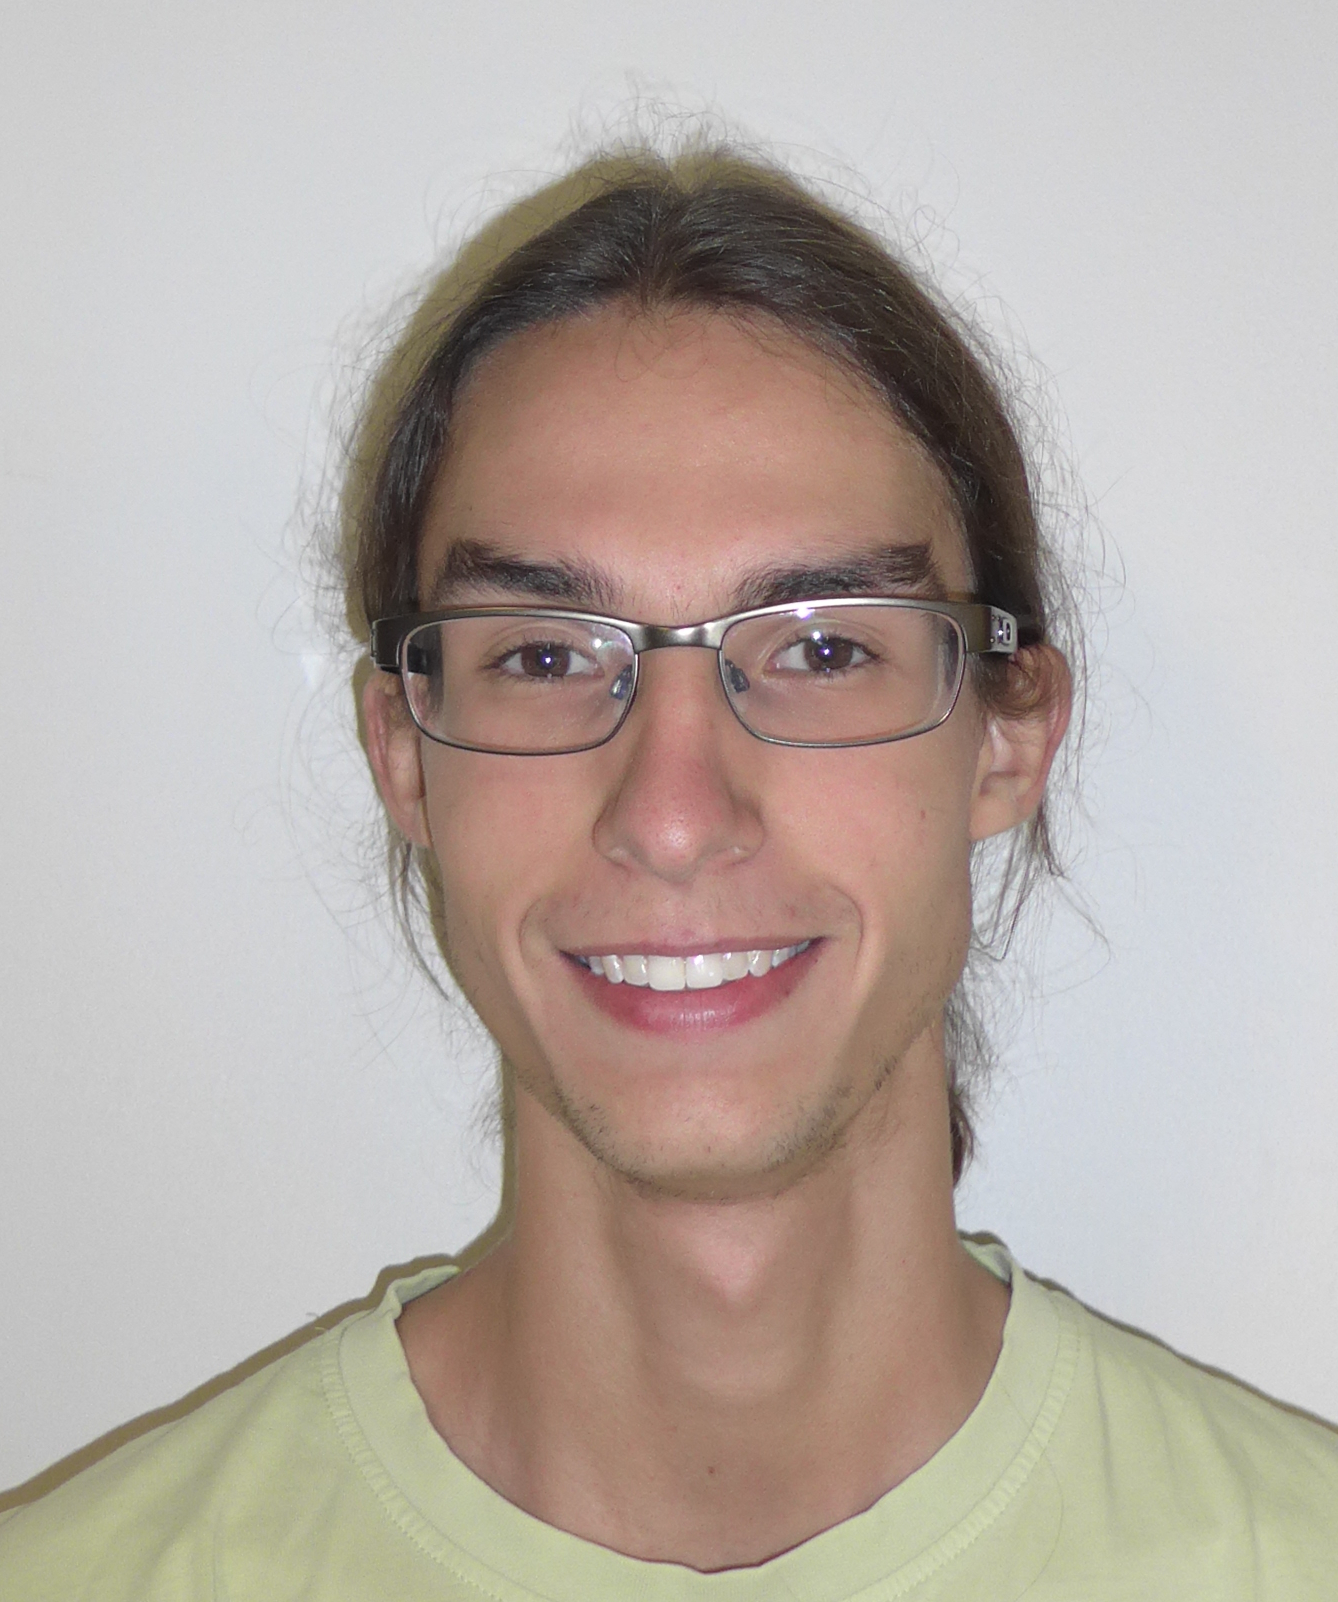
\includegraphics[scale=0.2]{pic}};
%\end{tikzpicture}

\begin{abstract}
	Abstract
\end{abstract}

\section{Objective}
Terrain is a topic of endless discussion in computer graphics. It has to cover a large area of the world and at the same time it has to provide enough details for close-up shots.
It is extremely time consuming to create a large-scale terrain that is also interesting when viewed closely. 

In this project I present a framework for generating terrain, from a coarse grained height map to vegetation generation. The focus lies on combining existing techniques for performing the single tasks.

Applications of procedural terrain include computer games, movies and geographic visualization and simulation.
The project was heavily inspired by a talk about "The Good Dinosaur" from Pixar Animation Studios.

\section{Related Work}
A lot of work has been done already in the field of generating height maps. There are in general three different approaches to this problem.
Generating the height map completely from scratch using perlin noise, fractals, voronoi regions, software agents or genetic algorithms are described in \cite{Doran.2010}, \cite{JacobOlsen.2004} and \cite{TeongJooOngRyanSaundersJohnKeyserJohnJ.Leggett.2005}. These models often lack realism because of the missing physically and geographic background. This is addressed in a second approach, hydraulic erosion models, as described in \cite{BedrichBenes.2007} and \cite{Mei.}. They start with existing height maps and increase the realism by simulating fluid to erode the terrain and forming rivers in the end. The other way is used in \cite{JeanDavidGenevauxEricGalinEricGuerinAdrienPeytavieBedrichBenes.2013}, here we start with a river network and build the terrain with respect to the river flow.
The last approaches copes with the lack of control in the previous described methods. They define the terrain by control features provided by the user, see \cite{FloraPonjouTasseArnaudEmilienMariePauleCaniStefanieHahmannAdrienBernhardt.2014} and \cite{Hnaidi.2010}.
On a 2D-scope, \cite{AmitPatel.2010} should be mentioned because it describes a complete new approach not using height map grids, but voronoi regions as base primitives.

After the terrain is created, it must be populated with vegetation. Rendering of grass is described in e.g. \cite{KurtPelzer.} and \cite{Boulanger.2005}. Trees must be generated first and for that, \cite{AdamRunionsBrendanLanePrzemyslawPrusinkiewicz.2007} and \cite{Weber.} should be mentioned.

\section{Overview}
TODO

\section{Polygonal Map}
TODO

\subsection{Graph Datastructure}
TODO

\subsubsection{Test}
TODO

\section{Terrain Features}
TODO

\section{Hydraulic Erosion}
TODO

\section{Vegetation}
TODO

\section{Conclusion and future work}
TODO

\bibliographystyle{IEEEtran}
%\bibliographystyle{alpha}
\bibliography{Paper}
\end{document}